\label{chap:Pipeline}

This chapter presents the complete computational pipeline developed for 
automated seismic phase picking and earthquake catalog generation. The workflow 
is structured into five principal stages: (0) data preprocessing, (1) phase 
picking, (2) event association, (3) hypocenter location and (4) magnitude 
estimation. Each stage builds upon its predecessor, collectively enabling a 
fully automated procedure for transforming continuous seismic waveforms into 
actionable seismological information suitable for both routine monitoring and 
retrospective catalog compilation.

\section{Data Preprocessing}

Prior to model inference, all daily continuous waveform segments undergo a 
unified preprocessing workflow to ensure consistency across stations, models, 
and time periods. This standardization is critical for reproducible results 
and optimal model performance.

\subsection{Sampling Rate Normalization}
The pretrained \ac{DL} models employed in this thesis were trained at a 
sampling rate of 100~Hz; consequently, all raw waveforms are resampled to this 
target frequency. Resampling at a fixed rate serves two essential purposes:
\begin{itemize}
  \item \textbf{Aliasing Prevention}: Proper anti-aliasing filters are applied 
  during decimation to prevent high-frequency artifacts from contaminating the 
  resampled signal
  \item \textbf{Architectural Compatibility}: The convolutional kernels and 
  receptive fields of the neural networks are calibrated for specific temporal 
  resolutions; mismatched sampling rates would alter the effective frequency 
  content perceived by the model
\end{itemize}

\subsection{Waveform Ingestion and Transformation}
Waveforms are retrieved from the OGS and EIDA continuous data archives in miniSEED 
(MSEED) format, the international standard for seismological waveform storage. 
The preprocessing chain, implemented using the ObsPy library, performs the 
following operations:
\begin{enumerate}
  \item \textbf{Parsing}: MSEED files are decoded into ObsPy Stream objects, 
  preserving metadata including station codes, channel identifiers, and timing 
  information
  \item \textbf{Detrending}: Linear and polynomial trends are removed to 
  eliminate DC offsets and instrumental drift
  \item \textbf{Merging}: Fragmented traces from the same channel are 
  concatenated, with gap handling strategies applied as appropriate
  \item \textbf{Array Conversion}: Processed waveforms are transformed into 
  NumPy arrays, providing memory-efficient, contiguous representations 
  suitable for GPU-accelerated batch inference
\end{enumerate}

This preprocessing pipeline ensures that the input dataset is temporally 
consistent, numerically stable, and aligned with the architectural requirements 
of modern \ac{DL}-based phase pickers.

\section{Phase Picking}

Seismic phase picking constitutes the foundational stage of the automated 
catalog generation pipeline. This task is performed using state-of-the-art 
\ac{DL} models, accessed through the SeisBench framework (\cite{SeisBench}),
specifically PhaseNet (\cite{PhaseNet}) and EQTransformer
(\cite{EQTransformer}), evaluated across 
three widely adopted benchmark datasets: INSTANCE, STEAD, and SCEDC. These 
models have emerged as the de facto standard in modern seismology due to their 
robustness, generalizability, and demonstrated capacity to outperform 
traditional picking algorithms such as \ac{STA/LTA} (\cite{STALTA}) and 
AIC-based methods, particularly under low signal-to-noise conditions.

\subsection{Advantages of Deep Learning Approaches}
\ac{DL}-based phase picking offers several fundamental advantages over 
conventional methods:
\begin{itemize}
  \item \textbf{Automatic Feature Learning}: End-to-end training enables 
  the extraction of discriminative features directly from raw waveforms, 
  eliminating the need for handcrafted signal descriptors and domain-specific 
  preprocessing

  \item \textbf{High Temporal Precision}: Modern architectures achieve 
  sub-sample accuracy in identifying P- and S-wave arrival times, often 
  matching or exceeding expert analyst performance

  \item \textbf{Noise Resilience}: Deep networks exhibit remarkable 
  robustness to noise, signal variability, and waveform distortion, enabling 
  consistent performance across diverse seismic networks and geological 
  settings

  \item \textbf{Computational Efficiency}: Optimized inference pipelines 
  support low-latency processing, making these models suitable for both 
  real-time monitoring and high-throughput retrospective analysis
\end{itemize}

These characteristics make \ac{DL}-based pickers ideal candidates for 
integration into operational earthquake monitoring systems and large-scale 
catalog generation workflows.

\subsection{PhaseNet}

PhaseNet (\cite{PhaseNet}) (Fig.~\ref{fig:phasenet}) is a fully convolutional neural network (CNN)
designed explicitly for seismic phase picking. Its architecture leverages a 
deep encoder-decoder structure with skip connections, enabling the learning of 
multiscale temporal features present in seismic waveforms. By applying stacks 
of convolutional layers with progressively increasing receptive fields, 
PhaseNet captures both fine-grained temporal transitions characteristic of 
impulsive P-wave onsets and broader waveform patterns associated with emergent 
S-wave arrivals.

\subsubsection{Architectural Characteristics}
The key architectural attributes of PhaseNet relevant to this work include:
\begin{itemize}
  \item \textbf{U-Net Topology}: The encoder-decoder structure with skip 
  connections preserves high-resolution temporal information while enabling 
  multi-scale feature extraction

  \item \textbf{Probabilistic Outputs}: The network produces continuous 
  probability distributions for P-wave, S-wave, and noise classes at each 
  time sample, enabling flexible threshold tuning for different operational 
  scenarios

  \item \textbf{End-to-End Training}: The model is trained directly on 
  raw three-component waveforms without requiring manual feature engineering, 
  achieving high sensitivity and specificity through exposure to large, 
  diverse training datasets

  \item \textbf{Computational Efficiency}: The purely convolutional 
  architecture enables efficient batch processing and GPU parallelization, 
  making it suitable for high-throughput HPC workflows
\end{itemize}

PhaseNet's strong generalization performance across independent datasets has 
established it as one of the most widely deployed \ac{ML} phase pickers in the 
seismological community.

\begin{figure}[h!]
  \centering
  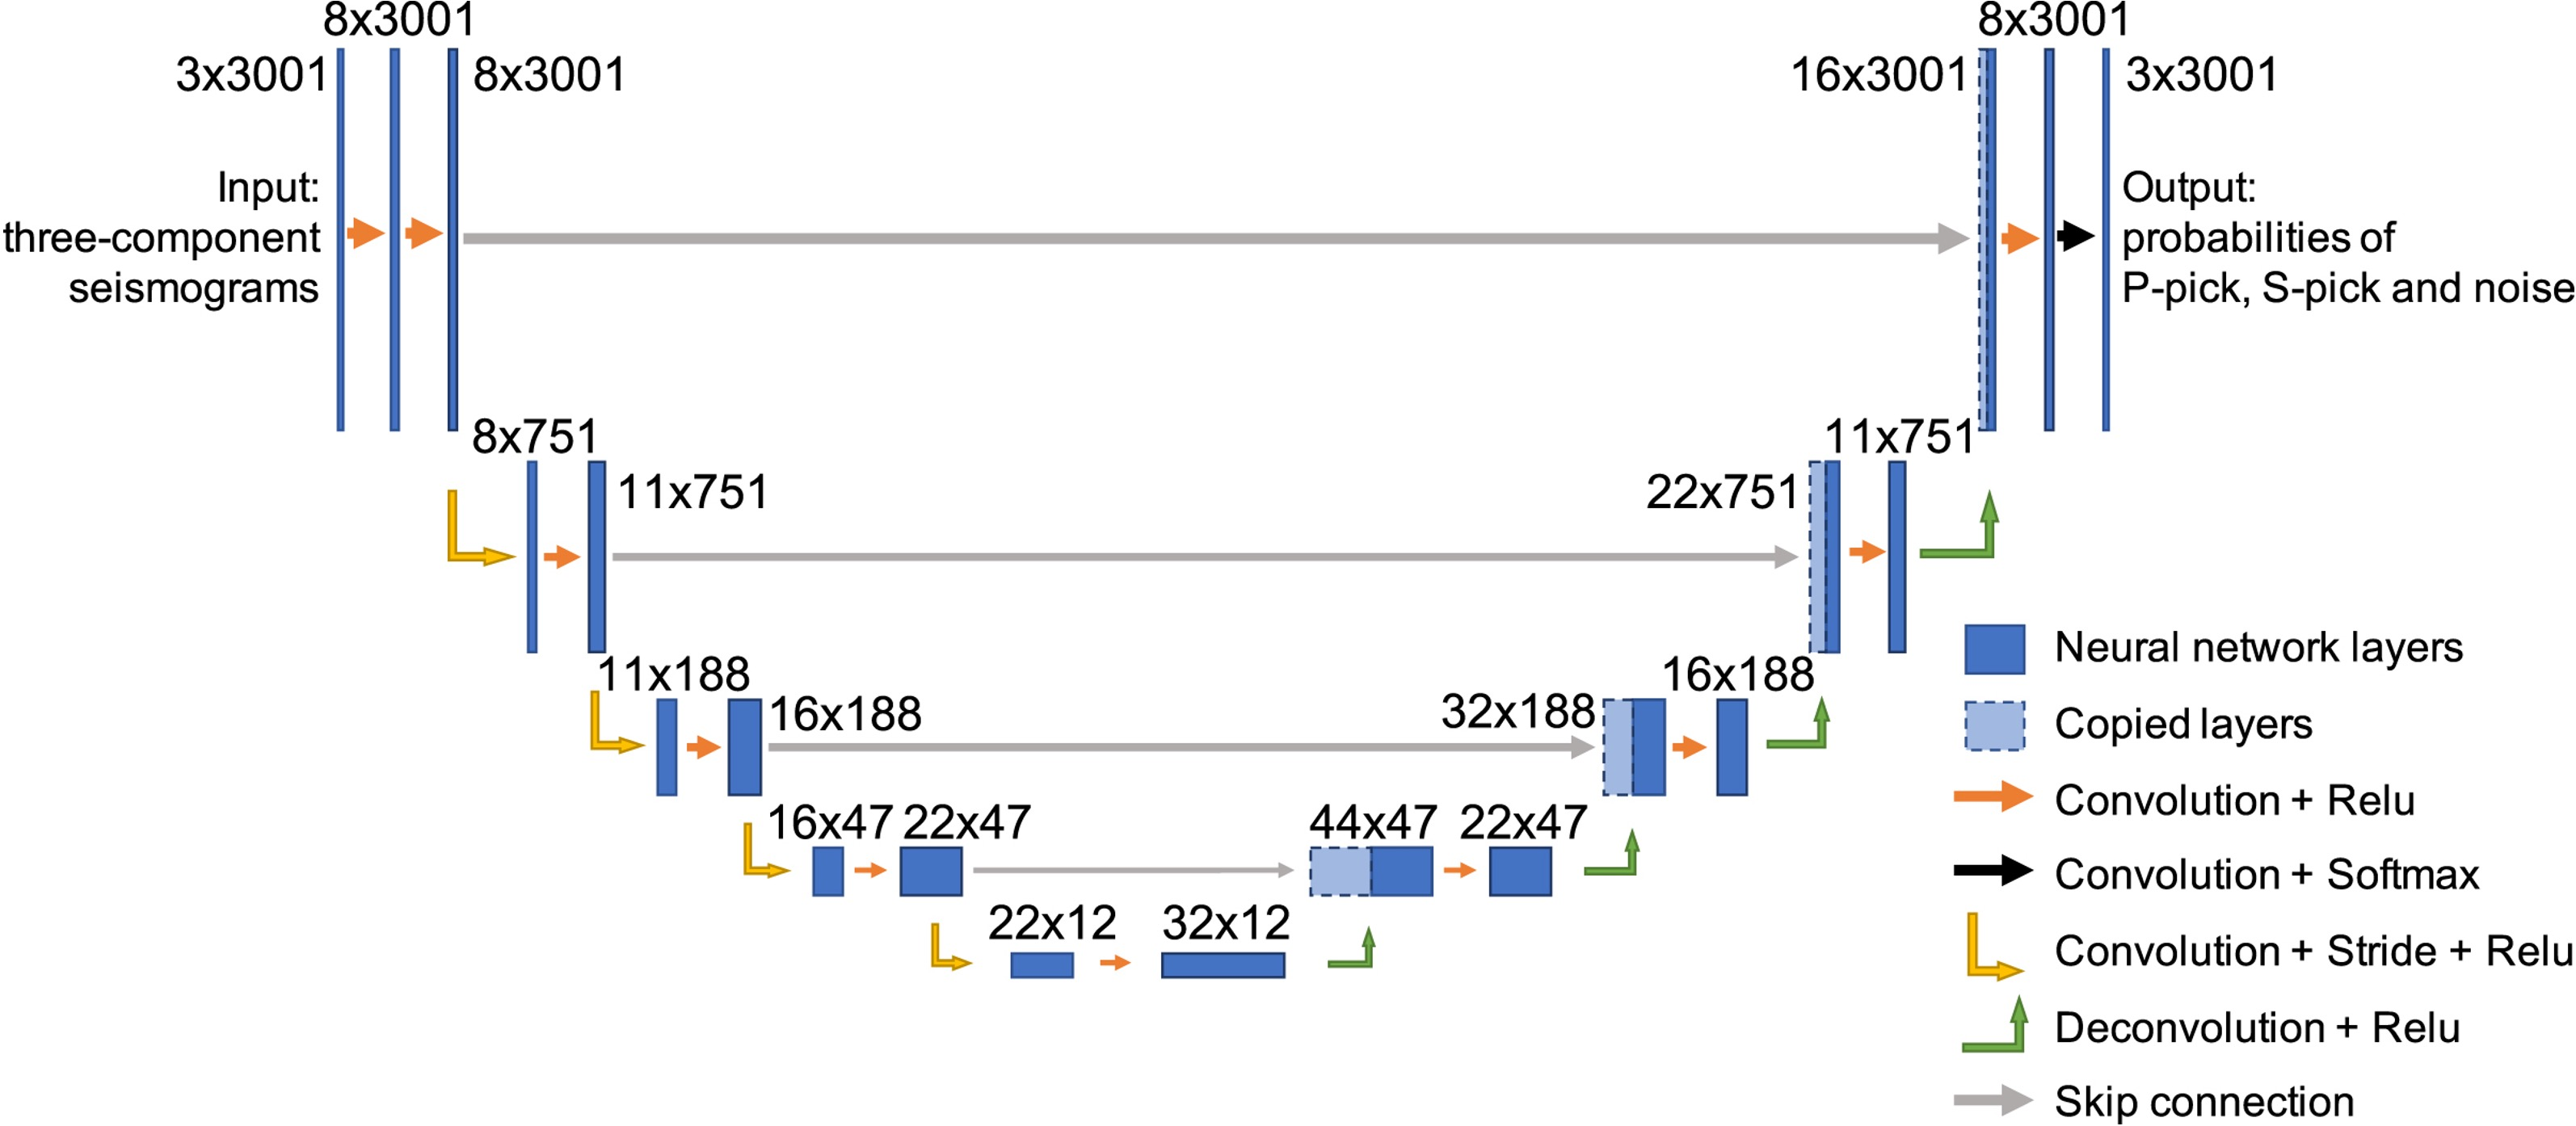
\includegraphics[width=\textwidth]{imgs/PhaseNet.jpg}
  \caption{Schematic of the PhaseNet architecture, illustrating the 
  hierarchical convolutional layers and output probability branches for P, S, 
  and noise classification. Image taken from \cite{PhaseNet}.}
  \label{fig:phasenet}
\end{figure}

\subsection{EQTransformer}

EQTransformer (\cite{EQTransformer}) (Fig.~\ref{fig:eqtransformer}) represents a state-of-the-art \ac{DL}
architecture for simultaneous earthquake detection and seismic phase picking. 
The model employs a hybrid Convolutional-Recurrent Neural Network (CNN-RNN) 
augmented with hierarchical attention mechanisms, enabling the extraction and 
interpretation of both local waveform features and long-range temporal 
dependencies in continuous seismic data. Crucially, the architecture performs 
three interrelated tasks simultaneously, event detection, P-wave arrival 
picking, and S-wave arrival picking, within a unified multi-task learning 
framework.

\subsubsection{Convolutional Encoder}
At the front end, EQTransformer employs a deep 1D convolutional encoder 
augmented with residual connections. This structure enables the extraction of 
both fine-scale and long-range temporal features from raw seismic waveforms. 
The convolutional kernels learn to recognize characteristic signatures 
including:
\begin{itemize}
    \item Impulsive P-wave onsets with sharp amplitude transitions
    \item Emergent S-wave arrivals with gradual energy buildup
    \item Amplitude modulations induced by path and site effects
\end{itemize}

Residual connections mitigate vanishing-gradient degradation and facilitate 
the training of deeper networks, thereby enabling the encoder to construct a 
multi-resolution hierarchy of features. This hierarchical representation is 
particularly important in seismology, where relevant information spans multiple 
time scales, from millisecond-level impulsive transients to several-second 
emergent phases.

\subsubsection{Bidirectional LSTM Layers}
Following the encoder, the model integrates a stack of bidirectional Long 
Short-Term Memory (BiLSTM) layers. LSTMs are particularly well-suited for 
sequential data due to their internal gating mechanisms that selectively 
retain or discard information over long temporal spans. The bidirectional 
structure allows the network to incorporate both past and future context, a 
capability essential for robust phase identification in noisy continuous 
waveforms. For instance, S-wave arrivals often follow complex coda patterns 
or overlapping microseismic bursts; a unidirectional model may misinterpret 
such signals, whereas a BiLSTM stabilizes predictions by integrating 
information from both temporal directions.

\subsubsection{Hierarchical Attention Mechanisms}
EQTransformer employs hierarchical attention modules that dynamically 
prioritize different waveform segments depending on the prediction task:
\begin{itemize}
  \item \textbf{Global Attention}: Enhances event detection by enabling the 
  model to identify broad-scale patterns such as energy bursts, emergent wave 
  trains, and characteristic spectro-temporal evolutions across the entire 
  input window

  \item \textbf{Local Attention}: Sharpens focus around potential arrival 
  windows, enabling fine-grained identification of P- and S-wave onsets. This 
  mechanism is analogous to an analyst zooming in on a candidate window once 
  an event has been recognized

  \item \textbf{Interpretability}: The attention weights provide insight 
  into which waveform segments most strongly influence the model's predictions, 
  offering a degree of interpretability uncommon in deep learning models
\end{itemize}

\subsubsection{Multi-Task Decoder Architecture}
The architecture concludes with three specialized decoder branches, each 
dedicated to a specific prediction task:
\begin{enumerate}
  \item \textbf{Event Detection}: Binary classification of whether an 
  earthquake signal is present in the input window
  \item \textbf{P-Phase Picking}: Precise temporal localization of P-wave 
  arrivals
  \item \textbf{S-Phase Picking}: Precise temporal localization of S-wave 
  arrivals
\end{enumerate}

Each branch outputs a continuous probability time series, effectively 
functioning as a smoothed likelihood estimator over the input window. Peaks in 
these probability functions correspond to predicted arrival times, enabling 
straightforward thresholding or peak-finding algorithms in downstream 
applications. This unified design allows simultaneous detection and picking 
within a single forward pass, an efficient alternative to multi-stage 
pipelines that employ separate event detectors and dedicated phase pickers.

\begin{figure}[h!]
  \centering
  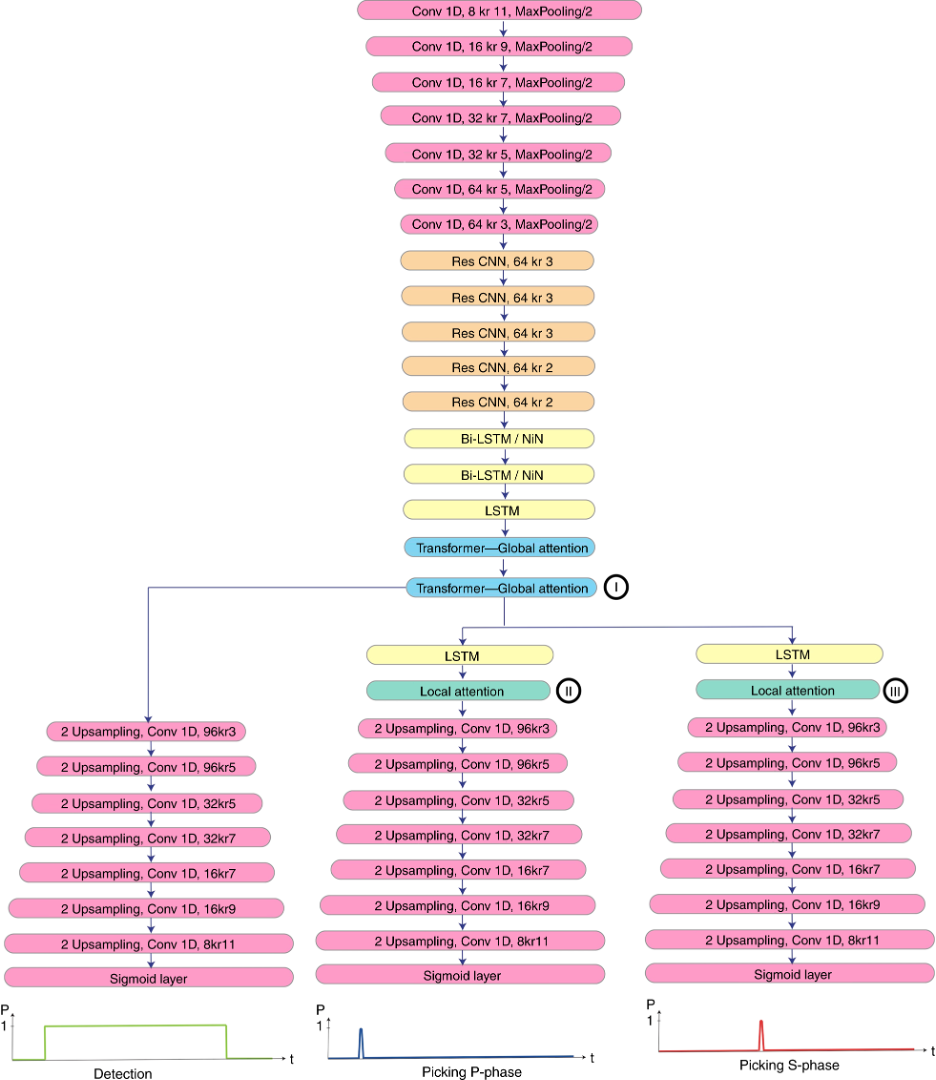
\includegraphics[width=\textwidth]{imgs/EQTransformer.png}
  \caption{Schematic of the EQTransformer architecture, illustrating the 
  convolutional encoder, BiLSTM layers, hierarchical attention modules, and 
  parallel decoder branches for event detection and phase picking. Image taken
  from \cite{EQTransformer}.}
  \label{fig:eqtransformer}
\end{figure}

\subsubsection{Outputs and Uncertainty Estimation}

The model produces three parallel probability sequences for each input window:
\begin{itemize}
  \item \textbf{Event Detection Probability}: A binary classification sequence 
  used to flag segments of continuous data that likely contain an earthquake 
  signal

  \item \textbf{P-Pick Probability}: A continuous sequence indicating the 
  model's confidence in the presence of a P-wave arrival at each time sample

  \item \textbf{S-Pick Probability}: An analogous sequence for S-wave arrivals, 
  typically exhibiting broader peaks due to the emergent nature of secondary 
  phases
\end{itemize}

Phase arrival times are extracted by locating the maximum probability within 
each respective sequence, subject to configurable detection thresholds. 
Additionally, the model supports Monte Carlo dropout-based uncertainty 
estimation, enabling the quantification of pick confidence through 
probabilistic sampling across multiple stochastic forward passes. This 
uncertainty quantification is particularly valuable in noisy or ambiguous 
scenarios, enabling automated filtering of low-confidence picks or 
prioritization of candidates for manual review.

\section{Event Association}

Following phase picking, the association stage groups individual P- and S-wave 
arrival detections into coherent earthquake events. This combinatorial problem 
becomes computationally challenging when processing large volumes of picks, 
particularly in regions with high seismicity rates or when using sensitive 
detection thresholds that produce numerous false positives. Two complementary 
association algorithms are employed in this pipeline: GaMMA, which adopts a 
probabilistic clustering approach, and PyOcto, which utilizes space-time 
partitioning.

\subsection{GaMMA}

GaMMA (\cite{GaMMA}) is a Python package designed for earthquake phase 
association as an unsupervised clustering problem within a probabilistic 
framework. The algorithm employs a Bayesian Gaussian Mixture Model (BGMM) to 
associate seismic phase picks with potential earthquake sources. To enhance 
computational efficiency, GaMMA utilizes the DBSCAN algorithm (\cite{DBSCAN}) 
to pre-cluster picks based on spatiotemporal proximity before applying the 
BGMM for refined association. This hierarchical approach enables effective 
processing of large datasets while maintaining high association accuracy.

The core functionality of GaMMA encompasses two primary objectives: (1) 
assigning individual phase picks to specific earthquake events, and (2) 
estimating source parameters including hypocenter location, origin time, and 
preliminary magnitude. These objectives are achieved through maximum likelihood 
estimation using the Expectation-Maximization (EM) algorithm. The probabilistic 
model describes the likelihood of observed picks belonging to different 
earthquake clusters as follows:
\begin{equation}
  \log p(\mathbf{X}|\phi, \mu, \Lambda, \mathbf{Z}) = \sum_{n=1}^{N} \log 
  \left( w_n\sum_{k=1}^{K} \phi_k \mathcal{N}\left(x_n|\mu_k, 
  \Lambda_k^{-1}\right) \right)
\end{equation}
where:
\begin{itemize}
  \item $\mathbf{X} = \{x_1, x_2, \ldots, x_N\}$ represents the set of observed 
  phase picks,
  \item $x_n = {t_n, \rho_n}$ is the feature vector for the $n$-th pick, 
  including its arrival time $t_n$ and amplitude $\rho_n$.
  \item $Z = \{z_1, z_2, \ldots, z_N\}$ denotes the set of latent variable 
  indicating the earthquake assignment for each pick.
  \item $\phi = \{\phi_1, \phi_2, \ldots, \phi_K\}$ are the mixture component 
  coefficients representing the prior probabilities of each earthquake.
  \item $\mu = \{\mu_1, \mu_2, \ldots, \mu_K\}$ are the mean vectors for each 
  earthquake cluster, representing expected pick features.
  \item $\Lambda = \{\Lambda_1, \Lambda_2, \ldots, \Lambda_K\}$ are the 
  precision matrices for each cluster, capturing the variability of pick 
  features around the mean.
  \item $\mathcal{N}(x_n|\mu_k, \Lambda_k^{-1})$ is the Gaussian probability 
  density function for pick $x_n$ given the parameters of the $k$-th earthquake 
  cluster.
  \item $w_n$ is a weight factor that can be used to adjust the influence of 
  each pick in the likelihood calculation.
\end{itemize}

The algorithm iterates between two key steps:

\subsubsection{Expectation Step (E-step)}
In this step, the algorithm computes the posterior probabilities 
($\gamma_{nk}$) that each pick $x_n$ belongs to earthquake cluster $k$, given 
the current estimates of the model parameters:
\begin{equation}
  \gamma_{nk} = \frac{\phi_k \mathcal{N}(x_n|\mu_k, \Lambda_k^{-1})}
  {\sum_{j=1}^{K} \phi_j \mathcal{N}(x_n|\mu_j, \Lambda_j^{-1})}
\end{equation}

\subsubsection{Maximization Step (M-step)}
In this step, the algorithm updates the model parameters ($\phi_k$, $\mu_k$, 
$\Lambda_k$) to maximize the expected log-likelihood of the observed picks,
weighted by the posterior probabilities computed in the E-step:
\begin{equation}
  \phi_k = \frac{1}{N} \sum_{n=1}^{N} \gamma_{nk}
\end{equation}
Estimating earthquake source parameters such as location and origin time 
involves maximizing the likelihood of the associated picks under the Gaussian 
mixture model. This is typically done using numerical optimization techniques, 
such as gradient descent or the Newton-Raphson method, to find the parameter 
values that maximize the log-likelihood function.
\begin{equation}
  \mu_k = \frac{\sum_{n=1}^{N} \gamma_{nk} x_n}{\sum_{n=1}^{N} \gamma_{nk}}
\end{equation}
\begin{equation}
  \Lambda_k = \left( \frac{\sum_{n=1}^{N} \gamma_{nk} (x_n - \mu_k)(x_n - \mu_k)^T}
  {\sum_{n=1}^{N} \gamma_{nk}} \right)^{-1}
\end{equation}
The E-step and M-step are repeated iteratively until convergence, which is
typically defined as a negligible change in the log-likelihood or model
parameters between successive iterations.

\subsection{PyOcto}

PyOcto (\cite{PyOcto}) is a high-throughput phase association algorithm 
designed for pick-heavy workflows in which modern \ac{DL} pickers produce 
large candidate sets that must be associated under strict runtime constraints. 
Its development is motivated by a practical trade-off: increasing picker 
recall typically improves event completeness, but also raises false-positive 
pick density and therefore the combinatorial burden of association. PyOcto 
targets this regime by prioritizing aggressive pruning and structured search, 
with the objective of preserving high recall while limiting runtime growth and 
controlling spurious associations.

\subsubsection{Search Mechanism in 4D Origin Space}
The core PyOcto strategy is to search event hypotheses in a four-dimensional 
origin space $(x, y, z, t)$ rather than directly enumerating pick 
combinations. The algorithm begins with coarse source-space nodes and evaluates 
whether each node is compatible with a sufficient set of picks under 
travel-time constraints. Candidate nodes are managed through a priority queue, 
and each extracted node triggers one of three actions:
\begin{enumerate}
  \item \textbf{Discard}: remove the node when compatibility criteria are not 
  met
  \item \textbf{Split}: partition the node into smaller subnodes when the 
  hypothesis remains plausible but is still too coarse
  \item \textbf{Localize/Create}: when criteria are satisfied at adequate 
  resolution, perform localization and instantiate an event candidate
\end{enumerate}
This branch-and-bound style search concentrates computation on promising 
regions of $(x, y, z, t)$ and avoids exhaustive evaluation of low-value 
hypotheses.

\subsubsection{Pruning and Early Stopping Criteria}
Early stopping is enforced through physically and operationally meaningful 
thresholds, including minimum total picks, minimum P picks, minimum S picks, 
and minimum station count with both phases. These criteria induce monotonic 
pruning: once a node fails lower-bound feasibility at a given scale, its 
descendants cannot recover feasibility under stricter partitioning, so the 
entire branch can be removed without loss of valid solutions under the same 
constraints. In addition, PyOcto can optionally filter distant stations during 
candidate evaluation, which reduces unnecessary matching operations in broad 
networks and improves runtime stability.

\subsubsection{Localization and Matching Refinement}
For nodes that pass pruning, PyOcto refines event parameters by optimizing a 
misfit objective based on the Euclidean distance transform (EDT) representation 
of pick residual structure (\cite{PyOcto}). The localization procedure uses an 
iterative split-and-select multiscale strategy: coarse hypotheses are 
progressively subdivided, and only subregions with improved objective values 
are retained. After each refinement step, inconsistent picks are treated as 
outliers and removed, while consistent picks are assigned to the candidate 
event. Once an event is accepted, its associated picks are removed from active 
nodes to limit duplicate reuse and reduce downstream ambiguity.

\subsubsection{Velocity Models and Travel-Time Querying}
PyOcto supports both homogeneous and 1D layered velocity models 
(\cite{PyOcto}). In practice, travel times are precomputed on grids and then 
queried through interpolation during search and localization. This design 
reduces per-candidate cost while retaining flexibility across network and 
regional settings. The homogeneous model generally yields faster execution with 
lower setup complexity, whereas the layered model often improves physical 
fidelity in stratified regions at the cost of higher preprocessing and query 
overhead; the choice therefore reflects a quality-runtime trade-off.

\subsubsection{Parallel System Design}
PyOcto is architected for parallel execution through overlapping base windows 
that can be processed concurrently and merged afterward (\cite{PyOcto}). The 
overlap mitigates boundary effects for events near window edges, while a 
deduplication stage reconciles duplicate candidates produced in neighboring 
windows. From a software perspective, PyOcto exposes a Python interface for 
workflow integration and orchestration, backed by a multithreaded C++ core for 
compute-intensive search and matching operations.

\subsubsection{Empirical Behavior and Practical Limitations}
Reported benchmarks indicate substantial acceleration relative to alternative 
association approaches, with runtime improvements of at least one order of 
magnitude and often above a factor of fifty under dense workloads 
(\cite{PyOcto}). For the 2014 Iquique sequence, the published results report 
an acceleration of at least $70\times$, with approximately 12--15~s/day 
compared with roughly 17~min/day and 25--26~min/day for reference alternatives 
(\cite{PyOcto}). These values should be interpreted as context-dependent 
performance indicators rather than universal constants, because runtime and 
quality depend on network geometry, pick noise, and parameter settings.

The same mechanism introduces identifiable trade-offs. Association quality is 
sensitive to threshold tuning; overly permissive settings increase false 
associations, while strict settings may suppress weak but valid events. Coarse 
search discretization can introduce quantization artifacts before refinement, 
and strongly heterogeneous velocity structures are only partially represented 
by simplified models. In very dense or noisy regimes, residual outlier 
contamination may still degrade assignment quality despite pruning.

\section{Hypocenter Location}

While associators such as GaMMA and PyOcto provide preliminary event locations 
as part of the clustering process, refining these hypocenters using dedicated 
location algorithms and detailed velocity models is essential for achieving the 
precision required for seismotectonic interpretation and catalog compilation.

\subsection{NonLinLoc}

For robust hypocenter determination, this pipeline employs the NonLinLoc 
(Non-Linear Location) package (\cite{NonLinLoc}). In contrast to linearized 
inversion methods (e.g., Hypo71 (\cite{Hypo71}), HypoInverse 
(\cite{HypoInverse})) that depend critically on the initial trial location and 
may converge to local minima in complex velocity structures, NonLinLoc performs 
a global search to estimate the complete posterior probability density function 
(PDF) of the hypocenter parameters $(x, y, z, T_0)$.

\subsubsection{Sampling Algorithms}
NonLinLoc implements two primary sampling strategies for exploring the 
four-dimensional solution space:
\begin{itemize}
  \item \textbf{Oct-Tree Search}: An adaptive grid refinement algorithm that 
  recursively subdivides cells containing high probability density, providing 
  efficient coverage of the solution space with computational cost proportional 
  to the posterior complexity

  \item \textbf{Metropolis-Gibbs Sampling}: A Markov Chain Monte Carlo (MCMC) 
  approach that generates samples from the posterior distribution, enabling 
  rigorous uncertainty quantification for complex, multimodal likelihood 
  surfaces
\end{itemize}

\subsubsection{Advantages of the Probabilistic Framework}
The NonLinLoc probabilistic framework offers several critical advantages for 
operational seismology:
\begin{itemize}
  \item \textbf{Complete Uncertainty Characterization}: The algorithm 
  provides a full description of location uncertainty through the posterior 
  PDF, producing appropriately scattered confidence clouds rather than 
  oversimplified ellipsoidal approximations when network geometry is 
  unfavorable or the problem is ill-constrained

  \item \textbf{Global Optimization}: Direct sampling of the misfit function 
  avoids the convergence issues inherent in gradient-based methods, ensuring 
  identification of the global maximum likelihood solution

  \item \textbf{3D Velocity Model Integration}: Seamless support for complex 
  three-dimensional velocity structures is essential for accurate locations 
  in structurally heterogeneous regions such as Northeastern Italy
\end{itemize}

\subsubsection{Implementation in the Pipeline}
In our workflow, the phase picks grouped by the associator are provided to 
NonLinLoc along with station metadata. Travel times are computed using a 1D 
layered velocity model appropriate for the study region, with travel-time 
lookup tables generated via a finite-difference Eikonal solver. The algorithm 
outputs three complementary location estimates for each event:
\begin{enumerate}
  \item \textbf{Maximum Likelihood Hypocenter}: The location corresponding to 
  the highest posterior probability
  \item \textbf{Expectation Hypocenter}: The probability-weighted centroid of 
  the posterior PDF
  \item \textbf{Posterior PDF}: The complete spatial probability density 
  function, enabling downstream uncertainty analysis
\end{enumerate}

\section{Magnitude Estimation}

The final stage of the catalog generation pipeline comprises the estimation of 
event magnitudes. This work focuses on the Local Magnitude ($M_L$), which 
which remains the standard magnitude scale for the OGS bulletin.

\subsection{Measurement Procedure}
Magnitude estimation is performed on the waveforms associated with each located 
event. The automated procedure encompasses four sequential stages:
\begin{enumerate}
    \item \textbf{Waveform Retrieval and Deconvolution}: Waveform segments 
  containing the event are extracted from the continuous archive. The 
  instrument response is removed through deconvolution to recover true ground 
  motion in displacement or velocity units

  \item \textbf{Wood-Anderson Simulation}: To comply with the classical 
  definition of $M_L$, the ground motion is convolved with the transfer 
  function of a standard Wood-Anderson torsion seismograph

  \item \textbf{Amplitude Measurement}: The maximum zero-to-peak amplitude 
  is measured on both horizontal components (N and E) of the simulated 
  Wood-Anderson traces within a time window following the S-wave arrival

  \item \textbf{Magnitude Computation}: The station magnitudes are computed 
  using a distance-dependent attenuation correction calibrated for the specific 
  region, then averaged across all contributing stations
\end{enumerate}

\subsection{Local Magnitude Formula}
The local magnitude ($M_L$) is computed following the standard formulation of
\cite{HuttonBoore1987}, applying the specific regional attenuation coefficients
and station correction terms calibrated for the OGS network (\cite{SMINO}).

